\chapter{Design and Experiments}
Summary of the experiment results and their details laid out in this section.
Neural network experiment logs are published online for more detailed examination, they are accessible by the url provided in the corresponding footnotes of this section.

\section{Training Specifications}
Training for traditional machine learning used in this project is fallows two step approach.
At the first part hyper-parameters for the model is selected by cross validation score then in the second part model is trained on entire dataset with the selected hyper-parameters.
Final model then evaluated on the test set.

There are many artificial neural networks used in both in benchmarking and the model selection.
Weights of the networks initialized by random except for the transfer learning models.
Model used in the transfer learning experiments initialized with the weighs pre-trained on imagenet~\cite{imagenet} dataset.
Each architecture is trained end-to-end using Adam~\cite{adam} optimizer with the standard parameters ($\beta_1 = 0.9$ \& $\beta_2 = 0.999$).
I used batch size of 64 for the training, and initial learning rate of 0.001 that decayed by the factor of 10 every time validation loss stagnates after an epoch.
Each image in the dataset is is downscaled to $224 \times 224$ size and normalized values to between zero to one.
Data augmentation is applied to minority class in the dataset to create a balanced dataset as explained in section \ref{sec:dataprocessing}.
Random cropping, changing saturation and horizontal flipping are set of augmentations chosen to create a balanced dataset.


\section{Benchmark Experiments}

\subsection{Random Forest Classifier and SVM}
Cross validation results of the random forest classifier found the fallowing hyper-parameters achieves the best performance:

\begin{itemize}
    \item Number of trees: 500
    \item Information gain criteria: Gini
    \item Number of max features: Square root
    \item Bootstrap: allowed
\end{itemize}

Cross validation for the support vector machine classifier runs suggested the fallowing hyper-parameters will achieve the best metrics:

\begin{itemize}
    \item Regularization parameter: 10
    \item Kernel: rbf
    \item Polynomial degree: 3
    \item Kernel coefficient $\gamma$: scale
    \item Tolerance: 0.001
\end{itemize}

Confusion matrix of these classifiers generated fallowing results.

\begin{figure}[H]%
    \centering
    \subfloat[Random forest]{{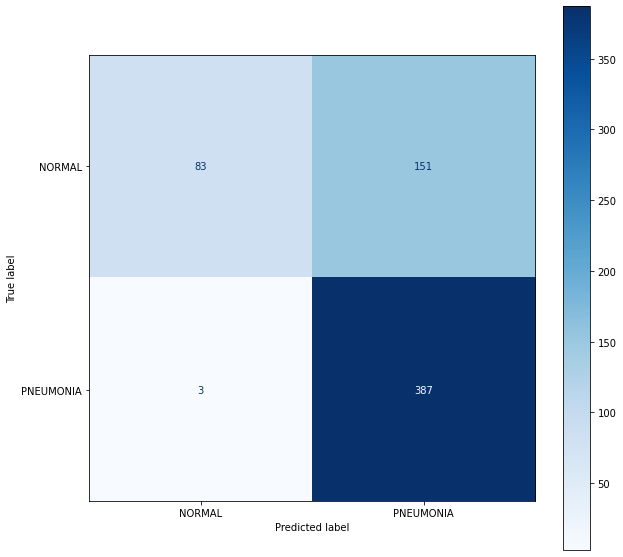
\includegraphics[width=.4\textwidth]{img/rf-confusion-matrix.png} }}%
    \qquad
    \subfloat[SVC]{{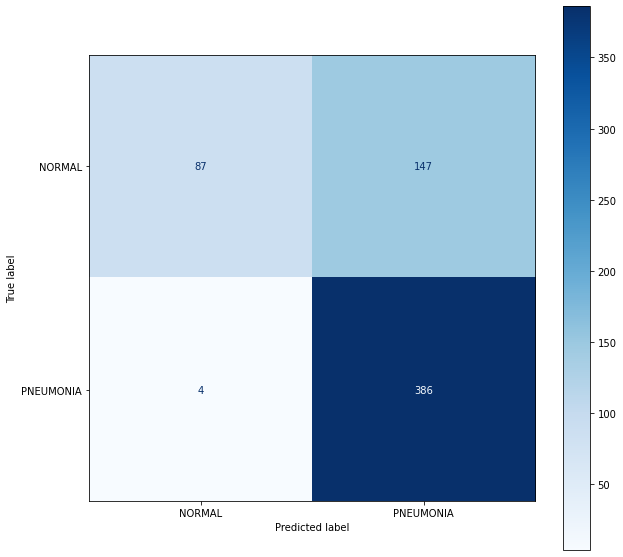
\includegraphics[width=.4\textwidth]{img/svm-confusion-matrix.png} }}%
    \caption{Confusion matrix of the classifiers.}%
    \label{fig:cmatrix}%
\end{figure}

\begin{table}[H]
    \centering
    \begin{tabular}{||c c c c c||} 
    \hline
    Classifier & Accuracy & Precision & Recall & f1\\ [0.5ex] 
    \hline\hline
    Random Forest & 0.7532 & 0.3547 & 0.9650 & 0.5187\\ 
    \hline
    SVC & 0.7580 & 0.3718 & 0.9560 & 0.5354\\
    \hline
    \end{tabular}
    \caption{Performance metrics for traditional machine learning algorithms.}
    \label{table:mlmetrics}
\end{table}

\subsection{LeNet-5}
\subsection{AlexNet}
AlexNet~\footnote{AlexNet Base:https://tensorboard.dev/experiment/PaBawCErSqG6zIef7JPq8g/}
balanced: https://tensorboard.dev/experiment/7b6W0tdHQQ2RINGt6cYbrA/

\subsection{VGGNet}
% vggnet https://tensorboard.dev/experiment/IbsPnocxSMKqNjmdJ3CdpA/
% vgg balanced https://tensorboard.dev/experiment/ABd8GrKdSXyzHgNPDngeEw/


\section{Custom NN Architecture}

\section{Transfer Learning}
% vgg https://tensorboard.dev/experiment/VxxyXkn6TaSMrgKnSP1low/
% vgg-balanced https://tensorboard.dev/experiment/c1zSx6N0QviARqCVIq3QMw/

\section{Interpreting Model Decisions}

% base (https://tensorboard.dev/experiment/p2mkNoLORACZlCXL2UQRbg)
% augmented (https://tensorboard.dev/experiment/dmQIbMeJQtqF70MhQQqySA)